\documentclass[a4paper]{article}
\usepackage{cmap}
\usepackage[utf8]{inputenc}
\usepackage[T2A]{fontenc}
\usepackage[english,russian]{babel} 
\usepackage[left=15mm, top=15mm, right=15mm, bottom=30mm, nohead, nofoot]{geometry}
\usepackage{blindtext}  % рыба-текст
\usepackage{graphicx}  % изображения
\usepackage{float} % плавающие объекты
\usepackage{wrapfig}  % изображения
\usepackage{tikz} % графика
\usepackage{mdframed} % рамки
\usepackage{xcolor} % определение цветов
\usepackage{nicefrac} % красивые дроби
\usepackage{cancel} % сокращение
\usepackage{amsmath,amsfonts,amssymb} % математический пакет
\usepackage{hyperref}  % гиперссылки
\usepackage{fancybox,fancyhdr} % хедер и футер
\usepackage{listings} % код
\usepackage[skip=2pt]{caption} % расстояние между подписью и картинкой
\pagestyle{fancy}
\fancyhf{}
\fancyhead[L]{Практическая работа №4}
\fancyhead[R]{\textit{Преобразование форм дискретных систем управления}}
\fancyfoot[C]{\thepage}
\headsep=4mm
\footskip=13mm
\setlength{\parindent}{0em}
\setlength{\parsep}{0em}
\setlength{\headheight}{12pt}
\setlength{\topmargin}{-38pt}
\setlength{\arraycolsep}{2pt}

\definecolor{urlcolor}{HTML}{3454D1}
\definecolor{linkcolor}{HTML}{3454D1}
\hypersetup{
    pdfstartview=FitH,
    linkcolor=linkcolor,
    urlcolor=urlcolor,
    colorlinks=true,
    pdftitle={Практическая работа №4},
    pdfauthor={Овчинников П.А.}
}

\definecolor{strings}{rgb}{0,0.6,0}
\definecolor{comments}{rgb}{0,0.3,0}
\definecolor{numbers}{rgb}{0.5,0.5,0.5}
\definecolor{keywords}{rgb}{0.09,0.61,0.95}
\definecolor{background}{rgb}{0.97,0.97,0.97}
\lstdefinestyle{codestyle}{
    backgroundcolor=\color{background},
    commentstyle=\color{comments},
    keywordstyle=\color{keywords},
    stringstyle=\color{strings},
    numberstyle=\tiny\color{numbers},
    basicstyle=\ttfamily\footnotesize,
    breakatwhitespace=false,
    breaklines=true,
    captionpos=b,
    inputencoding=utf8,
    keepspaces=true,
    numbers=left,
    numbersep=5pt,
    showspaces=false,
    showstringspaces=false,
    showtabs=false,
    tabsize=2,
    extendedchars=true,
    literate=
    {а}{{\cyra}}1
    {б}{{\cyrb}}1
    {в}{{\cyrv}}1
    {г}{{\cyrg}}1
    {д}{{\cyrd}}1
    {е}{{\cyre}}1
    {ж}{{\cyrzh}}1
    {з}{{\cyrz}}1
    {и}{{\cyri}}1
    {й}{{\cyrishrt}}1
    {к}{{\cyrk}}1
    {л}{{\cyrl}}1
    {м}{{\cyrm}}1
    {н}{{\cyrn}}1
    {о}{{\cyro}}1
    {п}{{\cyrp}}1
    {р}{{\cyrr}}1
    {с}{{\cyrs}}1
    {т}{{\cyrt}}1
    {у}{{\cyru}}1
    {ф}{{\cyrf}}1
    {х}{{\cyrh}}1
    {ц}{{\cyrc}}1
    {ч}{{\cyrch}}1
    {ш}{{\cyrsh}}1
    {щ}{{\cyrshch}}1
    {ъ}{{\cyrhrdsn}}1
    {ы}{{\cyrery}}1
    {ь}{{\cyrsftsn}}1
    {э}{{\cyrerev}}1
    {ю}{{\cyryu}}1
    {я}{{\cyrya}}1
    {А}{{\CYRA}}1
    {Б}{{\CYRB}}1
    {В}{{\CYRV}}1
    {Г}{{\CYRG}}1
    {Д}{{\CYR96}}1
    {Е}{{\CYRE}}1
    {Ж}{{\CYRZH}}1
    {З}{{\CYRZ}}1
    {И}{{\CYRI}}1
    {Й}{{\CYRISHRT}}1
    {К}{{\CYRK}}1
    {Л}{{\CYRL}}1
    {М}{{\CYRM}}1
    {Н}{{\CYRN}}1
    {О}{{\CYRO}}1
    {П}{{\CYRP}}1
    {Р}{{\CYRR}}1
    {С}{{\CYRS}}1
    {Т}{{\CYRT}}1
    {У}{{\CYRU}}1
    {Ф}{{\CYRF}}1
    {Х}{{\CYRH}}1
    {Ц}{{\CYRC}}1
    {Ч}{{\CYRCH}}1
    {Ш}{{\CYRSH}}1
    {Щ}{{\CYRSHCH}}1
    {Ъ}{{\CYRHRDSN}}1
    {Ы}{{\CYRERY}}1
    {Ь}{{\CYRSFTSN}}1
    {Э}{{\CYREREV}}1
    {Ю}{{\CYRYU}}1
    {Я}{{\CYRYA}}1
}
\lstset{style=codestyle}

\addto\captionsrussian{
  \renewcommand{\contentsname}
    {\centering Содержание}
}
\newcommand{\addsection}[1]{
    \phantomsection
    \addcontentsline{toc}{section}{#1}
    \section*{\centering #1}
}
\newcommand{\addsubsection}[1]{
    \phantomsection
    \addcontentsline{toc}{subsection}{#1}
    \subsection*{\centering #1}
}
\newcommand{\addsubsubsection}[1]{
    \phantomsection
    \addcontentsline{toc}{subsubsection}{#1}
    \subsubsection*{\centering #1}
}

\newmdenv[
    leftmargin = 0.5em,
    skipabove = 0.5em,
    skipbelow = 0.5em,
    linewidth = 1pt,
    rightline = false,
    topline = false,
    bottomline = false
]{quotebox}

\newlength{\tempheight}
\newcommand{\Let}{
\mathbin{\text{\settoheight{\tempheight}{\mathstrut}\raisebox{0.4\pgflinewidth}{
\tikz[baseline=0.5ex,line cap=round,line join=round] \draw (0,0) --++ (0.3em,0) --++ (0,2.3ex) --++ (-0.3em,0);
}}}}
\newcommand*\squared[1]{\tikz[baseline=(char.base)]{
            \node[shape=rectangle,draw,inner sep=4pt] (char) {#1};}}
\newcommand*\msquared[1]{\tikz[baseline=(char.base)]{
            \node[shape=rectangle,draw,inner sep=4pt] (char) {$\displaystyle #1$};}}
\newcommand\argmax[1]{\underset{#1}{\text{argmax}}}
\newcommand\argmin[1]{\underset{#1}{\text{argmin}}}
\renewcommand\max[1]{\underset{#1}{\text{max}}}
\renewcommand\min[1]{\underset{#1}{\text{min}}}
\newcommand{\at}{\biggr\rvert}
\newcommand{\shiftright}[3]{\makebox[#2][r]{\makebox[#1][l]{#3}}}
\newcommand{\e}{\;\text{e}}
\let\oldint\int
\def\int{\oldint\limits}
\DeclareRobustCommand{\divby}{%
  \mathrel{\vbox{\baselineskip.65ex\lineskiplimit0pt\hbox{.}\hbox{.}\hbox{.}}}%
}

\newcommand\NB{\textbf{N\kern-0.32em\textcolor{red}{B}}}

\begin{document}
\begin{titlepage}
    \begin{center}
        \includegraphics[width=0.18\textwidth]{~/Изображения/itmo_logo.png}\\[10pt]
        Федеральное государственное автономное образовательное \\ учреждение высшего образования \\[6pt]
        САНКТ-ПЕТЕРБУРГСКИЙ НАЦИОНАЛЬНЫЙ \\ ИССЛЕДОВАТЕЛЬСКИЙ УНИВЕРСИТЕТ ИТМО \\[16pt]
        Факультет систем управления и робототехники \vfill
        {\large Практическая работа №4} \\[0.5em]
        {\large \textbf{\MakeUppercase{Преобразование форм дискретных систем управления}}}\\[0.5em]
        Вариант №4
    \end{center}\vfill
    \begin{flushright}
        \begin{minipage}{0.3\textwidth}
            Студенты:\\339308, Дьячихин Д.Н. (1.1) \\ 368606, Овчинников П.А. (1.2) \\ 368731, Румянцев А.А. (1.2)\\[0.5em]
            Преподаватель: Семёнов Д.М.
        \end{minipage}
    \end{flushright}\vfill
    \begin{center}
        {\small Санкт-Петербург \\ 2024}
    \end{center}
\end{titlepage}
\setcounter{page}{2}
\addsection{Задание №1}
Дана каноническая модель дискретной системы в пространстве состояний с нулевыми начальными данными:
$$\begin{cases}
        x_{k+1} = Ax_k + Bu_k, \\
        y_k = Cx_k,
    \end{cases}$$
где $x_k \in \mathbb{R}^3, u_k \in \mathbb{R},$
$$A = \left[\begin{array}{rrr}
            0 & 1 & 0 \\ 0 & 0 & 1 \\ -0.7 & -0.1 & -0.3
        \end{array}\right],\quad B = \left[\begin{array}{rrr}
            -0.3 \\ -0.4 \\ 0.8
        \end{array}\right],\quad C = \begin{bmatrix}
        0 & 0 & 1
    \end{bmatrix}$$
Необходимо перейти к функциональной форме «вход-выход» и построить передаточную функцию системы.
\addsubsection{Выполнение задания}
Начнём с характеристического многочлена матрицы $A$:
$$a(\lambda) = \left| \lambda I - A \right| = \begin{vmatrix}
        \lambda & -1 & 0 \\ 0 & \lambda & -1 \\ 0.7 & 0.1 & \lambda + 0.3
    \end{vmatrix} = \lambda^3 + 0.3\lambda^2 + 0.1\lambda + 0.7$$
Определим систему многочленов, рекуррентно выводимых из характеристического многочлена $a(\lambda)$:
\begin{eqnarray*}
    a_{(1)}(A) &=& A^2+0.3A+0.1I \\
    a_{(2)}(A) &=& A+0.3I \\
    a_{(3)}(A) &=& I
\end{eqnarray*}
Получаем следующие матрицы:
$$a_{(1)}(A) = \left[\begin{array}{rrr}
            0.1 & 0.3 & 1 \\ -0.7 & 0 & 0 \\ 0 & -0.7 & 0
        \end{array}\right]\qquad a_{(2)}(A) = \left[\begin{array}{rrr}
            0.3 & 1 & 0 \\ 0 & 0.3 & 1 \\ -0.7 & -0.1 & 0
        \end{array}\right] \qquad a_{(3)}(A) = \begin{bmatrix}
        1 & 0 & 0 \\ 0 & 1 & 0 \\ 0 & 0 & 1
    \end{bmatrix}$$
Вспомним, что
$$a(\nabla)y_k = Ca_{(1)}(A)Bu_k + Ca_{(2)}Bu_{k+1} + \ldots + Ca_{(n)}(A)Bu_{k+n-1} = b(\nabla)u_k,$$
где $\nabla$ --- оператор сдвига вправо по времени.\\[0.5em]
Таким образом, находя $Ca_{(1)}(A)B = 0.28$, $Ca_{(2)}(A)B = 0.25$, $Ca_{(3)}(A)B = 0.8$, получаем уравнение в функциональной форме «вход-выход»:
$$y_{k+3}+0.3y_{k+2}+0.1y_{k+1}+0.7y_k = 0.8u_{k+2}+0.25u_{k+1}+0.28u_k$$
Теперь найдём передаточную функцию системы, используя модель «вход-выход»:
$$W(\lambda) = \frac{0.8\lambda^2+0.25\lambda+0.28}{\lambda^3+0.3\lambda^2+0.1\lambda+0.7} = \frac{8\lambda^2 + 2.5\lambda + 2.8}{10\lambda^3 + 3\lambda^2 + \lambda + 7}$$
Аналогично можно найти передаточную функцию исходной системы в пространстве состояний:
$$W(\lambda) = C(\lambda I - A)^{-1}B = \begin{bmatrix}
        0 & 0 & 1
    \end{bmatrix}\left[\begin{array}{rrr}
            \lambda & -1 & 0 \\ 0 & \lambda & -1 \\ 0.7 & 0.1 & \lambda + 0.3
        \end{array}\right]^{-1}\left[\begin{array}{r}
            -0.3 \\ -0.4 \\ 0.8
        \end{array}\right] = \frac{8\lambda^2 + 2.5\lambda + 2.8}{10\lambda^3 + 3\lambda^2 + \lambda + 7}$$
\newpage
\addsection{Задание №2}
Дана функциональная модель дискретной системы в форме «вход-выход»:
$$y_{k+3}-0.8y_{k+2}+0.3y_{k+1}-0.1y_k = 0.1u_{k+2}-0.2u_{k+1}-0.05u_k,$$
где $y_k, u_k \in \mathbb{R}.$ Необходимо перейти к канонической модели в форме пространства состояний.
\addsubsection{Выполнение задания}
Для представления системы «вход-выход» в канонической форме пространства состояний функциональную модель необходимо записать в виде:
$$\begin{cases}
        x_{k+1} = Ax_k + Bu_k, \\
        y_k = Cx_k,
    \end{cases}$$
$$\text{где } A = \left[\begin{array}{rcc}
            0.8 & 1 & 0 \\ -0.3 & 0 & 1 \\ 0.1 & 0 & 0
        \end{array}\right],\quad B=\left[\begin{array}{r}
            0.1 \\ -0.2 \\ -0.05
        \end{array}\right], \quad C = \begin{bmatrix}
        1 & 0 & 0
    \end{bmatrix}$$
\addsection{Задание №3}
Дана передаточная функция устойчивой линейной системы:
$$W(\lambda) = \frac{\lambda + 3}{\lambda^2 + 3\lambda + 1}$$
\begin{itemize}
    \item Построить переходную функцию данной системы в среде.
    \item Найти передаточную функцию дискретной системы по методу Эйлера.
    \item Получит оценку на шаг дискретизации, при котором дискретная система будет устойчивой.
    \item Построить переходную функцию полученной дискретной системы для двух разных шагов дискретизации: в первом случае дискретная система устойчива, во втором - неустойчива. Сравнить результаты исходной системы.
    \item Найти передаточную функцию дискретной системы, соответствующей исходной, по методу Тастина.
    \item Построить переходную функцию полученной дискретной системы. Сравнить с поведением исходной системы.
\end{itemize}
\addsubsection{Выполнение задания}
Построим график переходной функции с помощью функции \texttt{stepplot} в среде MATLAB. График переходной функции представлен на рис. \ref{fig:stepplot}.
\begin{figure}[H]
    \centering
    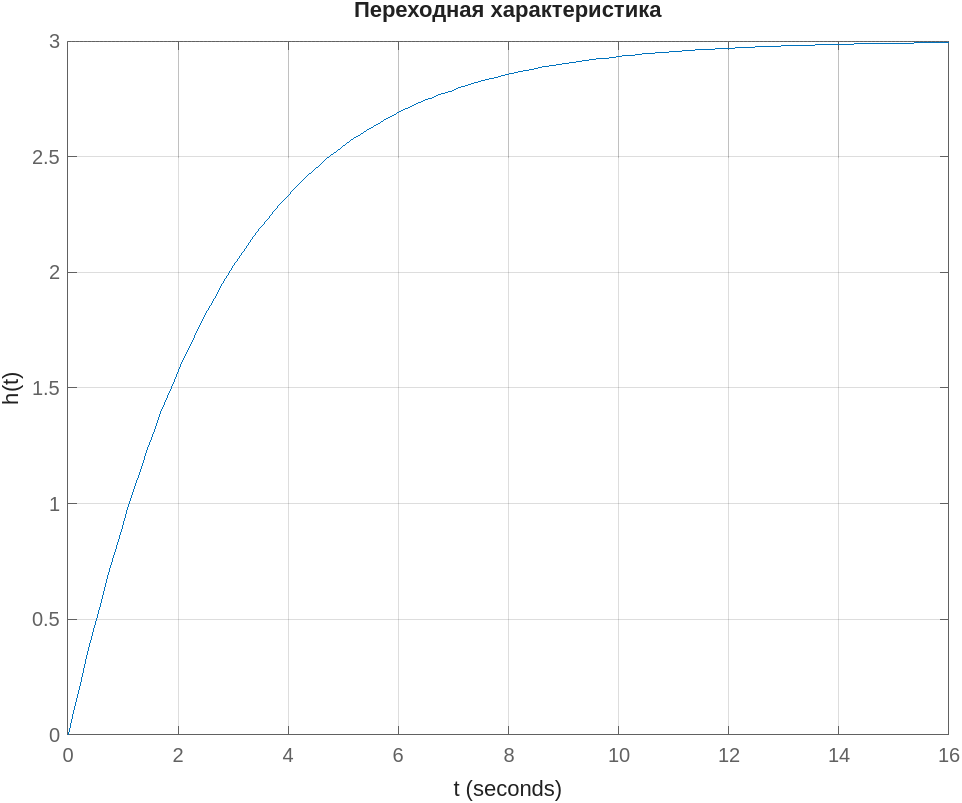
\includegraphics[width=0.356\textwidth]{sources/stepplot.png}
    \caption{График переходной функции}
    \label{fig:stepplot}
\end{figure}
Найдём передаточную функцию дискретной системы по методу Эйлера:
$$W_\text{д}(\lambda) = W_\text{н}\left( \frac{\lambda - 1}{h} \right) = \frac{\frac{\lambda - 1}{h} + 3}{\frac{(\lambda - 1)^2}{h^2} + \frac{3\lambda - 3}{h} + 1} = \frac{\frac{\lambda - 1 + 3h}{h}}{\frac{(\lambda - 1)^2 +3h\lambda - 3h + h^2}{h^2}} = \frac{h^2\lambda - h^2 + 3h^3}{h\lambda^2 - 2h\lambda + h + 3h^2\lambda - 3h^2 + h^3} =$$
$$= \frac{h\lambda + 3h^2 - h}{\lambda^2 + (3h - 2)\lambda + h^2 - 3h + 1}$$
Оценим шаг дискретизации, при котором получившаяся дискретная система будет устойчивой:
$$h < \min{i}\frac{2\left| Re(\lambda_i) \right|}{\left| \lambda_i \right|^2} \approx 0.6667.$$
Если взять шаг, больший оцененному, то система даст неустойчивую аппроксимацию. Чтобы это проверить, построим графики переходной функции полученной дискретной системы для двух разных шагов дискретизации: $h = 0.5667$ и $h = 0.7667$. Графики представлены на рис. \ref{fig:stepplot_discrete}.
\begin{figure}[H]
    \centering
    \begin{minipage}{0.356\textwidth}
        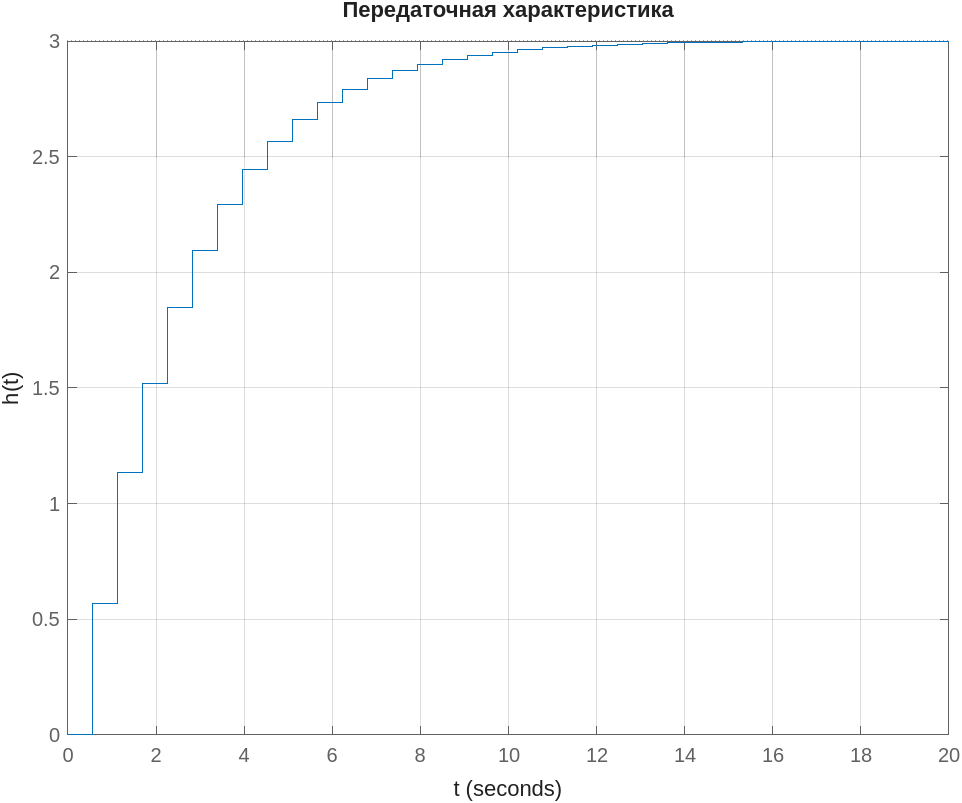
\includegraphics[width=1\textwidth]{sources/discrete_0.5667.png}
        \caption*{$h = 0.5667$}
    \end{minipage}
    \hspace{2em}
    \begin{minipage}{0.356\textwidth}
        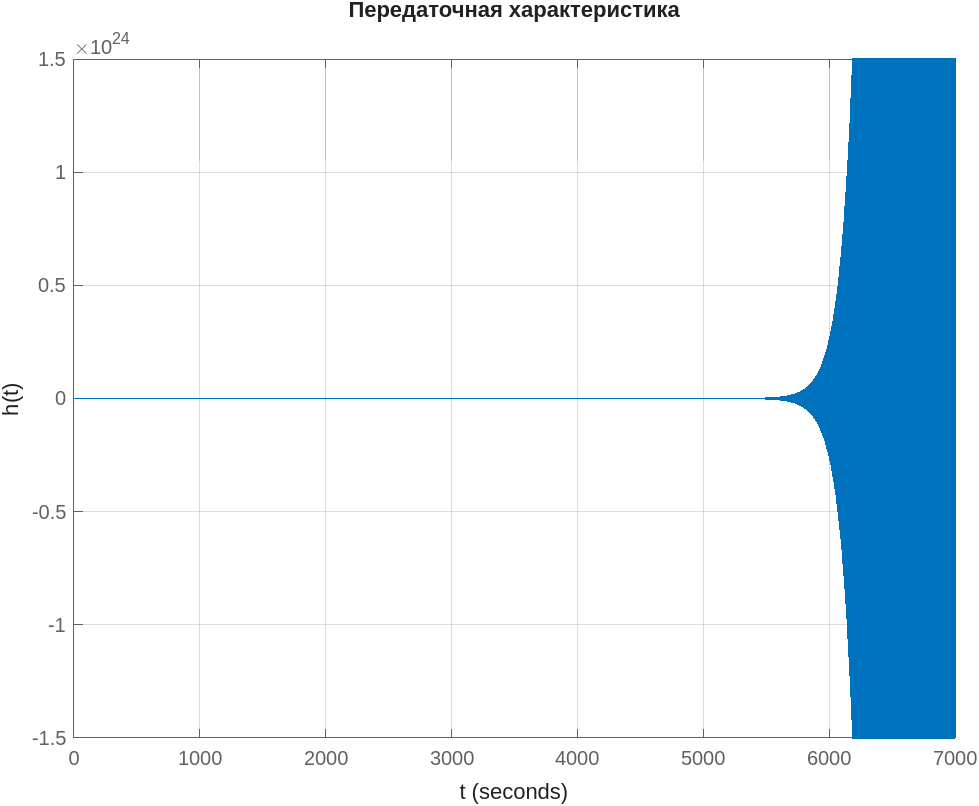
\includegraphics[width=1\textwidth]{sources/discrete_0.7667.png}
        \caption*{$h = 0.7667$}
    \end{minipage}
    \caption{Графики переходной функции дискретной системы, полученной по методу Эйлера}
    \label{fig:stepplot_discrete}
\end{figure}
Теперь найдём передаточную функцию дискретной системы по методу Тастина:
$$W_\text{д}(\lambda) = W_\text{н}\left( \frac{2}{h}\left[ \frac{\lambda - 1}{\lambda + 1} \right] \right) = \frac{\frac{2}{h}\left[ \frac{\lambda - 1}{\lambda + 1} \right] + 3}{\left( \frac{2}{h}\left[ \frac{\lambda - 1}{\lambda + 1} \right] \right)^2 + \frac{6}{h}\left[ \frac{\lambda - 1}{\lambda + 1} \right] + 1} = \frac{\frac{2\lambda - 2}{h(\lambda + 1)} + 3}{\frac{4(\lambda - 1)^2}{h^2(\lambda + 1)^2} + \frac{6h\lambda - 6h}{h(\lambda + 1)} + 1} = $$
$$ = \frac{h\left( \lambda + 1 \right)\left( 2\lambda - 2 + 3h\left( \lambda + 1 \right) \right)}{4(\lambda - 1)^2 + 6h^2\lambda(\lambda + 1) - 6h^2(\lambda + 1) + h^2(\lambda + 1)^2} =$$
$$= \frac{3 h^{2} \lambda^{2} + 6 h^{2} \lambda + 3 h^{2} + 2 h \lambda^{2} - 2 h}{4\lambda^2 - 8\lambda + 4 + 6h^2\lambda^2 + \cancel{6h^2\lambda} - \cancel{6h^2\lambda} - 6h^2 + h^2\lambda^2 + 2h^2\lambda + h^2} = \frac{\left( 3 h^{2}+2h \right)\lambda^2 + 6h^2\lambda + 3h^2 - 2h}{\left( 7h^2 + 4 \right)\lambda^2 + \left( 2h^2 - 8 \right)\lambda - 5h^2+ 4}$$
Построим график переходной функции полученной дискретной системы по методу Тастина с тем шагом дискретизации, при котором система, полученная методом Эйлера, была неустойчивой, т.е. с шагом $h = 0.7667$. График представлен на рис. \ref{fig:stepplot_tustin}.
\begin{figure}[H]
    \centering
    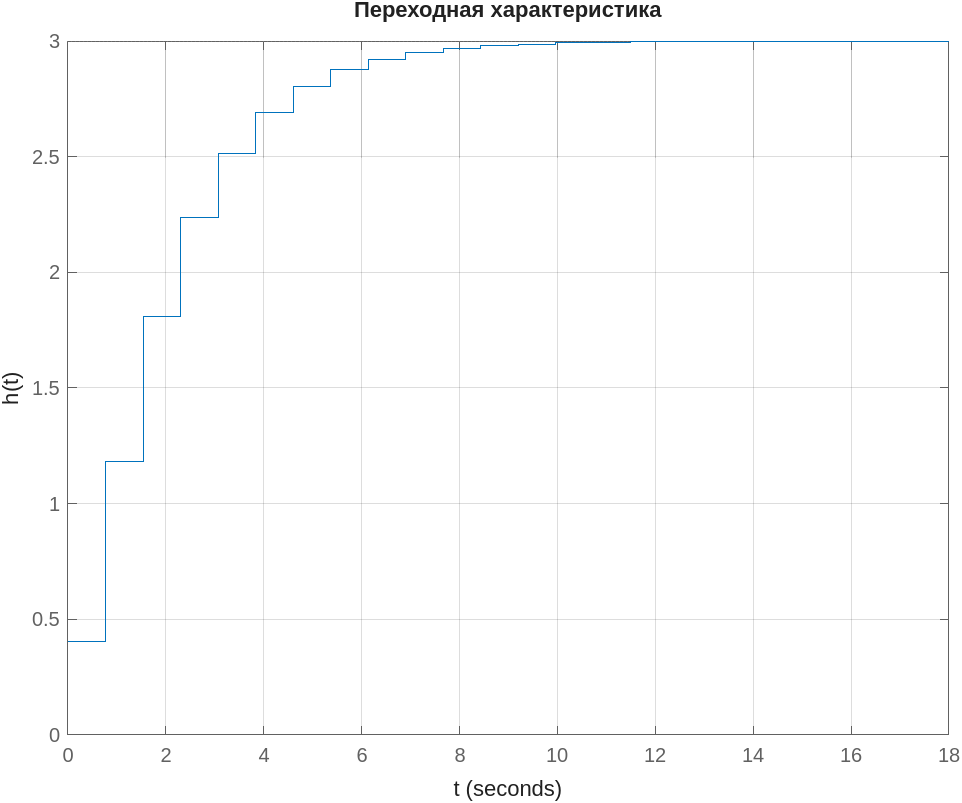
\includegraphics[width=0.356\textwidth]{sources/discrete_0.7667_tustin.png}
    \caption{График переходной функции дискретной системы по методу Тастина с шагом $h = 0.7667$}
    \label{fig:stepplot_tustin}
\end{figure}
Итак, дискретная система по методу Тастина остаётся устойчивой в отличие от системы по методу Эйлера.
\addsection{Вывод}
В ходе выполнения практической работы были изучены методы преобразования форм дискретных систем управления. Мы научились работать с функциональными формами системы, а также с преобразованием их в пространство состояний. Также изучили методы Эйлера и Тастина, позволяющие найти передаточную функцию дискретной системы по известной передаточной функции непрерывной системы, и понятие устойчивости дискретных систем. Также мы научились строить графики переходных функций дискретных систем управления.
\end{document}